\chapter{Literature Review}

The following chapter blah blah blah...

\section{Data Stream}

Golab and Ozsu define data stream as "a real-time, continuous, ordered (implicitly by arrival time or explicitly by timestamp) sequence of items. It is impossible to control the order in which items arrive, nor is it feasible to locally store a stream in its entirety". \cite{golab2003issues}

\subsection{Comparison to a Database Management System (DBMS)}

Historically, data has been stored into database management systems (DBMS) where it was later analysed the assumption being that there would be enough disk space to contain the data. This approach fits many purposes but recently applications started "feeling the need" to analyse rapidly changing data on-the-fly.

This has brought on an advent of data stream processing. Several stream-processing frameworks have emerged such as Apache Storm \cite{ApacheStorm}, Apache Spark \cite{ApacheSpark}, Yahoo S4 \cite{YahooS4}, and Onyx \cite{Onyx}. These frameworks, usually ran on a cluster, provide the user with abstractions which greatly simplify writing a real-time data stream processing application.

Whereas DBMSs excel at getting an exact answer to a query, data streams usually provide an approximate answer. The answer is approximate because it is usually correct only within a certain window of time, the query is simplified because it can only be ran in one pass, or because it is used with a sampling rate which does not include all events. A typical data stream analysis using windows and sampling is depicted in figure \ref{fig:stream}.

The assumption behind using a time window is that users are most likely interested in the most recent events. That way they can  react to change quickly. Sampling on the other hand is used to reduce the number of events used for a query. \cite{Gaber:2005:MDS:1083784.1083789}

\begin{figure}[!htb]
	\centering
	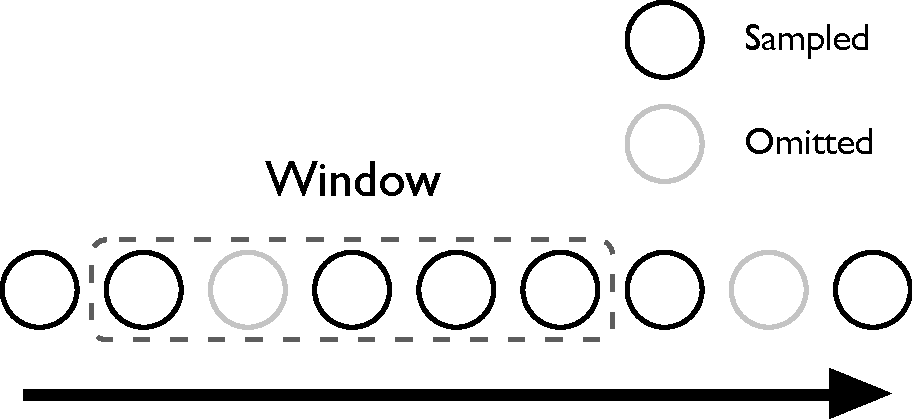
\includegraphics[scale=0.5]{pdf/stream.pdf}
	\caption{Stream Querying.}
	\label{fig:stream}
\end{figure}

Even though the answer might only be approximate it can have great value because the query is answered at the right time. Furthermore, even though the query may run only on a subset of data it is still possible to detect trends or system failures. For example, Twitter are using Apache Storm to run real-time analysis on millions of events per second for their analytics product. \cite{Solovey}

In research, several techniques have been developed to enable real time data stream mining. For example, the MOA environment \cite{Bifet:2010:MMO:1756006.1859903} which enables real time machine learning using the WEKA machine learning workbench \cite{Holmes1994}.

\section{Apache Storm}

Apache Storm is an open source distributed real-time computation system. Storm was Originally created by Nathan Marz while working at BackType. \cite{NathanAbout} BackType was later acquired by Twitter which is when Storm became open source. Storm was incubated into Apache with version 0.9.1 and became a top-level Apache project in September 2014.

Storm was developed to run on top of a cluster where nodes execute components of a computation in parallel.

\subsection{Dependencies}

Storm has five major dependencies:

\begin{description}
	\item[Apache Zookeeper] \hfill \\
	Apache Zookeeper \cite{ApacheZookeeper} is an open source server that allows reliable distributed coordination. Storm uses Apache Zookeeper to maintain state which is then read and written to by nodes of a Storm cluster. More detail on how Storm uses Zookeeper is given in section \ref{subsec:zookeeper}.
	\item[Apache Thrift] \hfill \\
	Apache Thrift \cite{ApacheThrift} is a cross-language framework for developing services. It allows you to write a definition file for services and data types required by your application and automatically generates interface code which supports remote procedure calls and serialisation of the data types.
	\item[Apache Kryo] \hfill \\
	Apache Kryo \cite{ApacheKryo} is a serialisation library. It is used by Storm to serialise objects when sent over the network between nodes of a cluster.
	\item[Netty] \hfill \\
	Netty \cite{Netty} is an asynchronous event-driven network application framework. Storm utilises Netty to send intra-cluster messages. Thus when a node produces a result to be consumed by another node of the cluster it sends a message over the network using the TCP protocol implemented in Netty.
	\item[LMAX Disruptor] \hfill \\
	LMAX Disruptor \cite{LMAXDisruptor} is a high-performance data structure used to exchange data between concurrent threads. It uses a lock-free implementation of a ring buffer which components of a Storm program running on the same node a cluster use to exchange messages.
\end{description}

Storm works well with sister projects such as Apache Kafka \cite{ApacheKafka} and Apache HBase \cite{ApacheHBase}. Apache Kafka is a messaging broker that is often used as the missing link between producers and consumers of a cluster. Apache HBase is a big data-store that allows real time random reads and writes modelled after Google's Bigtable project. \cite{Bigtable}

Storm is reportedly used by 81 companies listed on their website \cite{https://storm.apache.org/documentation/Powered-By.html} and possibly many others. Storm's popularity is one of the reasons why it was chosen for this project. Moreover, we believe that the concepts used in Storm (explained further in section \ref{sec:concepts}) apply to many different situations and many applications can be easily adapter to work on Storm.

There has been research into how to optimise computations running on a Storm cluster. \cite{Chatzistergiou:2014:FHN:2661829.2661882} looked at how to reconfigure the job by reallocating component tasks to minimise communication cost. 

There has been effort to port Hadoop to multi-core in \cite{Kumar:2013:HSD:2536274.2536314} (Hone) and \cite{ranger2007evaluating} (Phoenix). However, there has not been effort to port Storm or any other real time data stream framework to multi-core.

Running a real time data stream framework on multi-core has its own set of challenges, different to running it on a distributed system. 

\todo{What research has there been on Storm}

\section{Ports to Multi-core}

\section{Similar Efforts}

\todo{Has anyone ported Storm somewhere}

\todo{Real time on multi-core}

\todo{What has been ported}

\section{Summary}